
\begin{center}
\Huge
Proportionalitet og recap. om vækst
\end{center}
\section*{Recap. om vækst}
\stepcounter{section}

Vi har beskæftiget os med tre vigtige væksttyper; lineær vækst, eksponentiel vækst og nu potensvækst. Vi husker på, at en lineær funktion er en funktion $f$ med forskrift
\begin{align*}
f(x) = a\cdot x +b,
\end{align*}
en eksponentialfunktion $g$ er en funktion på formen
\begin{align*}
g(x) = b\cdot a^x,
\end{align*}
og en potensfunktion er en funktion $h$ på formen 
\begin{align*}
h(x) = b\cdot x^a.
\end{align*}
Eksempler på hver af de tre funktionstyper kan ses af Fig. \ref{fig:linekspot}
\begin{figure}[H]
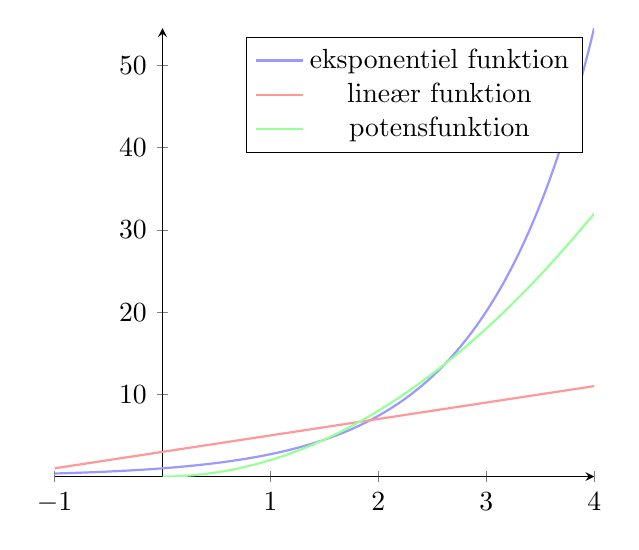
\begin{tikzpicture}
\begin{axis}[axis lines = middle, ymin=0,xmax = 4,xmin = -1]
\addplot[color=blue!40,samples = 1000,thick] {exp(x)};
\addplot[color=red!40,samples = 1000,thick] {2*x+3};
\addplot[color=green!40, samples = 1000, domain = 0:4,thick] {2*x^2};
\legend{eksponentiel funktion, lineær funktion, potensfunktion}
\end{axis}
\end{tikzpicture}
\caption{Eksempler på lineær funktion, eksponentiel funktion og potensfunktion.}
\label{fig:linekspot}
\end{figure}
I alle tre væksttyper er det muligt at finde en entydig funktion af væksttypen, der går gennem to punkter. Formlerne for at finde $a$ og $b$ kaldes for topunktsformlerne, og vi repeterer her, hvordan man finder $a$. Konstanten $b$ kan så findes tilsvarende ved at løse en simpel ligning. 
Den lineære funktion $f(x)=ax+b$, der går gennem punkterne $(x_1,y_1)$ og $(x_2,y_2)$ har hældning 
\begin{align*}
a = \frac{y_2-y_1}{x_2-x_1}.
\end{align*}
Den eksponentialfunktion $g(x) = b\cdot a^x$, der går gennem punkterne $(x_1,y_1)$ og $(x_2,y_2)$ har fremskrivningsfaktor 
\begin{align*}
a = \sqrt[x_2-x_1]{\frac{y_2}{y_1}}.
\end{align*}
Den potensfunktion $h(x) = b\cdot x^a$, der går gennem punkternen $(x_1,y_1)$ og $(x_2,y_2)$ har følgende udtryk for $a$.
\begin{align*}
a = \frac{log(y_2)-\log(y_1)}{\log(x_2)-\log(x_1)}.
\end{align*}
\section*{Regression}
\stepcounter{section}
Vi har i forbindelse med de tre væksttyper set regression på et datasæt for hver type af vækst. Det er dog ikke helt klart, hvordan vi i fald vi støder ind i virkelighedsnær data afgør, hvilken type regression, vi skal bruge. Lad os sige, at vi har datasættet, der fremgår af Tabel \ref{tab:papvaegt}
\begin{table}[H]
\begin{tabular}{c|c|c|c|c|c|c|c|c|c|c}
$x$ & 1 & 2 & 3 & 4 & 5 & 6 & 7 & 8 & 9 & 10 \\ \hline
$V(x)$ & 78.1 & 319.9 & 720.5 & 1280.4 & 2000.5 & 2881.1 & 3918.4 & 5119.4 & 6480.6 & 8001.6
\end{tabular}
\caption{Vægt af papirkvadrater med bredde $x$, hvor bredden er i meter og vægten er i gram.}
\label{tab:papvaegt}
\end{table}
Uden yderligere information om, hvor data kommer fra er der ikke andet for end at prøve forskellige regressionstyper og se, om regressionen passer godt på datasættet. På Fig. \ref{fig:reg} fremgår alle tre regressioner på datasættet
\begin{figure}[H]
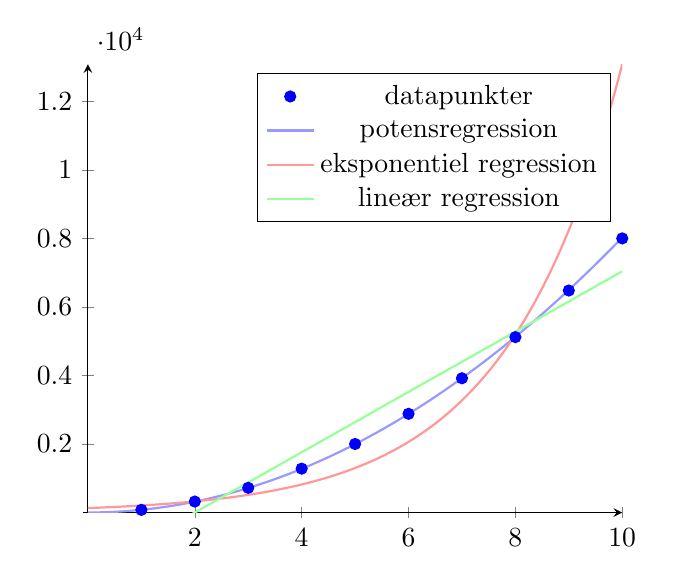
\begin{tikzpicture}
\begin{axis}[axis lines = middle, xmin = -0.1,ymin = -0.1]
\addplot[only marks,color = blue]  coordinates{(1,78.1)(2,319.9)(3,720.5)(4,1280.4)(5,2000.5)(6,2881.1)(7,3918.4)(8, 5119.4)(9, 6480.6)( 10, 8001.6)};
\addplot[color = blue!40, samples = 1000, thick, domain = 0:10] {78.913*x^(2.0075)};
\addplot[color = red!40, samples = 1000, thick, domain = 0:10] {128.89*(1.5874^x)};
\addplot[color = green!40, samples = 1000, thick, domain = 0:10] {880.15*x-1760.8};
\legend{datapunkter,potensregression,eksponentiel regression, lineær regression}
\end{axis}
\end{tikzpicture}
\end{figure}
Betragter vi regressionerne, ser det klart ud til at potensregression passer bedst på datapunkterne, men det er ikke altid sikkert, at det er så klart som i dette tilfælde. Mere generelt skal vi have information om, hvad den underliggende forklarende model til det, vi har målt på er. I dette tilfælde måler vi på vægten af papirkvadrater som funktion af bredden. Arealet af et papirkvadrat er $A(x) = K\cdot x^2$, hvor ,$x$ er bredden og $K$ er en passende konstant. Derfor giver det god mening at en potensfunktion $b\cdot x^a$, hvor $a\approx 2$ beskriver vægten af papirkvadraterne som funktion af bredden. 
\section*{Ligefrem og omvendt proportionalitet}
\stepcounter{section}
\begin{defn}[Ligefrem proportionalitet]
To variable $x$ og $y$ siges at være \textit{ligefrem proportionale} eller blot proportionale, hvis $y = a\cdot x$. Konstanten $a$ kaldes for \textit{proportionalitetsfaktoren} 
\end{defn}
\begin{defn}[Omvendt proportionalitet]
To variable $x$ og $y$ siges at være \textit{omvendt proportionale}, hvis $x\cdot y = k$.
\end{defn}
Hvis to variable er omvendt proportionale, er der en potenssammenhæng mellem dem, da $x\cdot y = k$ medfører, at $y = k\cdot x^{-1}$.
\begin{exa}
Lad os betragte et rektangel med areal $10$. Så er længden og bredden af rektanglet omvendt proportionale, da $b\cdot l = 10$
\end{exa}
\section*{Opgave 1}
Find en lineær funktion, en eksponentialfunktion og en potensfunktion, der går gennem følgende par af punkter:
\begin{align*}
&1)\  (2,2)  \textnormal{ og }(3,3)\\
&2)\  (1,5)  \textnormal{ og }(6,100)\\
&3)\  (1,7)  \textnormal{ og }(2,9)\\
\end{align*}
\section*{Opgave 2}
Lav selv potensregression på datasættet fra Tabel \ref{tab:papvaegt} og bestem, hvad et papirkvadrat på 20$m^2$ vejer. Hvad er vægten af papir per kvadratmeter i følge regressionen?
\section*{Opgave 3}
Hvilke af følgende variabelsammenhænge er proportionale, omvendt proportionale eller ingen af delene
\begin{align*}
&1) \  y = \frac{1}{x} &&2) \  x\cdot y = 27    \\
&3) \ \frac{y}{x} = 27 &&4) \  y=x^2   \\
&5) \ 2y = 3x &&6) \ 10x^3 = x^2y    \\ 
\end{align*}